%____________________WEEK 2_____________________________%
\newpage
\section{Tuần 2}
\subsection{Quy trình xây dựng chương trình AI}

- Quy trình xây dựng một chương trình AI bắt đầu từ việc thu thập dữ liệu thô. Sau đó \textbf{tiền xử lý} để thu được dữ liệu sạch. Tiếp đến, \textbf{huấn luyện mô hình} trên dữ liệu đó và \textbf{đánh giá mô hình} thu được. Hình 1 tóm tắt quy trình này:

\begin{figure}[H]
    \centering
    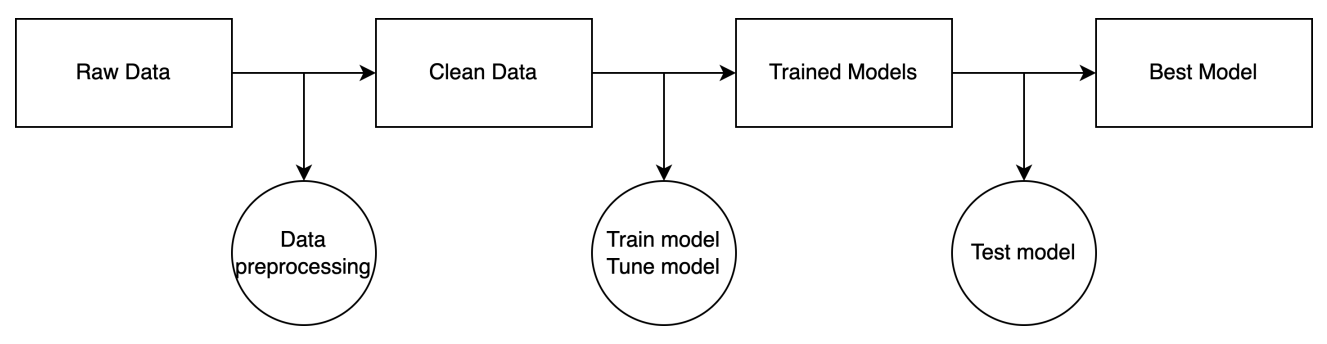
\includegraphics[width=1\linewidth]{img/QuyTrinhAI.png}
    \caption{Quy trình xây dựng một chương trình AI}
    
\end{figure}
\subsection{Tiền xử lý (Data preprocessing)} 
- Quá trình tiền xử lý dữ liệu \cite{data_pre} là bước quan trọng để biến đổi dữ liệu thô trở thành dữ liệu phù hợp cho quá trình huấn luyện của một mô hình AI. Một số quy trình tiền xử lý dữ liệu có thể kể đến bao gồm:
\begin{itemize}
    \item Làm sạch dữ liệu (Data cleaning)
    \item Tích hợp dữ liệu (Data integration)
    \item Thu giảm dữ liệu (Data reduction)
    \item Biến đổi dữ liệu (Data transform)
\end{itemize}
\begin{enumerate}
    \item \textbf{Làm sạch dữ liệu (Data cleaning): } Là quy trình loại bỏ các dữ liệu sai lệch, thiếu sót hoặc không phù hợp khỏi tập dữ liệu. Dữ liệu thô thường có xu hướng không đầy đủ, bị nhiễu và không toàn vẹn dữ liệu. Việc làm sạch dữ liệu sẽ giúp ta xử lý vấn đề trên. Ví dụ như xóa hàng loạt cột dữ liệu trống hoặc không có giá trị hay xóa các giá trị ngoại lai (các giá trị quá cao hoặc quá thấp so với các giá trị khác).
    \item \textbf{Tích hợp dữ liệu (Data integration):} Là quy trình hợp nhất các dữ liệu khác nhau từ nguồn khác nhau thành một tập dữ liệu duy nhất nhằm tránh việc dư thừa và làm mất đi tính toàn vẹn của dữ liệu trong tập dữ liệu. Ví dụ với một công ty có hai loại dữ liệu, một loại để theo dõi bán hàng và một loại dùng để theo dõi khách hàng. Để phân tích hiệu quả bán hàng, ta cần phải kết hợp cả hai dữ liệu này thành một tập dữ liệu duy nhất.
    \item \textbf{Thu giảm dữ liệu (Data reduction):} Là quy trình loại bỏ những thuộc tính dư thừa của dữ liệu thô mà không làm ảnh hưởng hay làm mất những thông tin quan trọng. Ví dụ với tập dữ liệu của một siêu thị gồm các danh mục sản phẩm trong siêu thị và số lượng giao dịch hàng ngày. Có thể thấy rằng tập dữ liệu này khá lớn và việc khai phá cũng tốn rất nhiều thời gian, dẫn đến việc phân tích dữ liệu này trở nên bất khả thi. Như vậy quy trình thu giảm dữ liệu là rất cần thiết.
    \item \textbf{Biến đổi dữ liệu (Data transform):} Là quy trình biến đổi dữ liệu từ dạng này sang dạng khác để phù hợp với quá trình khai phá dữ liệu. Ví dụ như chuyển đổi nhiệt độ từ độ C sang độ F hay chuyển đổi số điểm từ thang điểm 10 sang thang điểm 4 của một học sinh.
\end{enumerate}
- Sau khi tiền xử lý, tùy thuộc vào từng bài toán mà ta sẽ chia dữ liệu đã xử lý thành nhiều tập dữ liệu để sử dụng cho các bước tiếp theo. Một số cách chia thường được sử dụng:
\begin{itemize}
    \item Tập huấn luyện (Training sets), tập xác thực (Validation sets) và tập kiểm thử (Test sets)
    \item Chia dữ liệu theo thời gian (time series segmentation)
\end{itemize}
\begin{enumerate}
    \item \textbf{Tập huấn luyện (Training sets), tập xác thực (Validation sets) và tập kiểm thử (Test sets):} Đây là cách chia dữ liệu rất phổ biến. Ta chia dữ liệu thành 3 phần khác nhau gồm: Tập huấn luyện dùng để huấn luyện mô hình, tập xác thực dùng để điều chỉnh các tham số của mô hình và tập kiểm thử dùng để đánh giá hiệu suất của mô hình.
    \item \textbf{Chia dữ liệu theo thời gian (time series segmentation):} Với cách chia dữ liệu này, ta sẽ chia dữ liệu thành các tập dữ liệu khác nhau theo thời gian. Điều này sẽ giúp ích cho việc phân tích liên quan đến các xu hướng hoặc các biến động theo thời gian.
\end{enumerate}
\subsection{Huấn luyện mô hình (Train model/Tune model)}
\subsubsection{Cách mô hình dự đoán}
- Quy trình dự đoán của mô hình là một quy trình toán học được xây dựng để dự đoán hoặc ước lượng các giá trị đầu ra dựa trên đầu vào cụ thể bằng cách phân tích các mẫu trong một tập hợp dữ liệu đầu vào nhất định.
\\- Quá trình huấn luyện của một mô hình dự đoán thông thường bao gồm các bước sau:
\begin{itemize}
    \item \textbf{Chuẩn bị dữ liệu đầu vào:} Trước khi mô hình có thể dự đoán kết quả, ta cần chuẩn bị dữ liệu đầu vào, khởi tạo trọng số ngẫu nhiên cho các kết nối giữa các nút. Bước đầu cần phải thu thập dữ liệu đầu vào, điều này bao gồm hoạt động tiền xử lý dữ liệu (chuẩn hóa, mã hóa và chuyển đổi dữ liệu thành định dạng phù hợp) và sắp xếp các dữ liệu thành một tập dữ liệu duy nhất. 
    \item \textbf{Truyền thuận} (Forward propagation): Dữ liệu được truyền qua các lớp (lớp đầu vào, lớp ẩn và lớp đầu ra) trong neural network, sử dụng activation function để tính toán đầu ra dựa vào dữ liệu và trọng số hiện tại. 
    \item \textbf{Tính toán đầu ra:} Các dữ liệu được đưa qua neural network để huấn luyện mô hình qua nhiều vòng lặp (gọi là epochs), trọng số của mô hình được cập nhật để giảm thiểu hàm mất mát (Loss function). 
    \item \textbf{Đánh giá đầu ra:} Đầu ra được đánh giá bằng cách so sánh với giá trị thực tế hoặc nhãn đã biết trước (đối với bài toán có giám sát). Điều này giúp đánh giá hiệu suất của mô hình và xác định mức độ chính xác của dự đoán
\end{itemize}
\subsubsection{Ví dụ về mạng neural network cơ bản}
\begin{itemize}
    \item \textbf{Đặt vấn đề:} Xây dựng 1 mạng neural network để dự đoán đầu ra của toán tử AND, với 2 input là chân trị của A và B.\\
    Bảng chân trị của A, B và A AND B:
    \begin{table}[H]
    \centering
    \begin{tabular}{|c|c|c|}
    \hline
    \textbf{A} & \textbf{B} & \textbf{A AND B} \\ \hline
    0 & 0 & 0 \\ \hline
    0 & 1 & 0 \\ \hline
    1 & 0 & 0 \\ \hline
    1 & 1 & 1 \\ \hline
    \end{tabular}
    \end{table}
    \item \textbf{Mô hình neural network:}
    Ta sẽ xây dựng một neural network (thực chất là một perceptron) với input layer có 2 nút và output layer có 1 nút như sau:
    \begin{figure}[H]
        \centering
        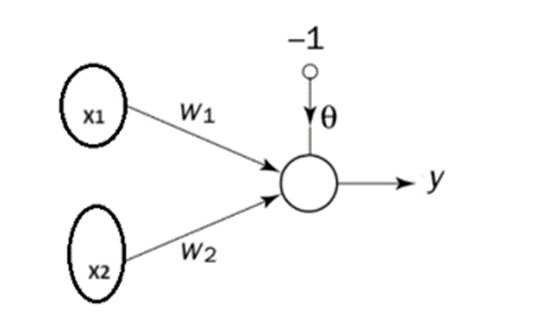
\includegraphics[width=0.5\linewidth]{perceptron.png}
        \caption{Neural network biểu diễn được toán tử AND}
        
    \end{figure}
    \item \textbf{Các bước huấn luyện mô hình neural network:}
    \begin{enumerate}
    \item \textbf{Khởi tạo:} Ban đầu, \textbf{trọng số} (weight) ($w_1, w_2$)  và \textbf{ngưỡng} (threshold)($\theta$) được gán các giá trị ngẫu nhiên (thông thường là trong đoạn [-0,5; 0,5])
    \item \textbf{Kích hoạt:}
    Ở lần học thứ \texttt{p} với đầu vào $x_1, x_2$, ta tính toán output như sau:
    \begin{center}
        \large $Y_{p} = \sigma(x_{1}w_{1}+x_{2}w_{2}-\theta)$
    \end{center}
        Trong đó:
        \begin{itemize}
        \item $x_{1}, x_{2}$: đầu vào
        \item $w_{1}, w_{2}$: trọng số tương ứng với mỗi đầu vào
        \item $\theta$: ngưỡng phân loại (classification threshold)
        \item $\sigma(x)$: hàm kích hoạt - ta dùng hàm bước (step function)
        \begin{center} 
        \begin{align*}
        \sigma(x)= \left\{
        \begin{aligned}
        1 \hspace{0.3cm} if \hspace{0.3cm} x \ge  0\\
        0 \hspace{0.3cm} if \hspace{0.3cm} x > 0
        \end{aligned}
        \right.
        \end{align*}
        \end{center}
        
        \end{itemize}
    
    \item \textbf{Cập nhật trọng số:}
    \begin{center}
        \large ${w_{i}}_{(p+1)} =  {w_{i}}_{(p)} + {\Delta w_{i}}_{(p)}$
    \end{center}
        Trong đó:
        \begin{itemize}
        \item ${w_{i}}_{(p+1)}$: trọng số của lần học thứ \texttt{p+1}
        \item ${w_{i}}_{(p)}$: trọng số của lần học thứ \texttt{p}
        \item ${\Delta w_{i}}_{(p)}$: sự thay đổi khi cập nhật trọng số
        \end{itemize}
        Quy tắc điều chỉnh trọng số: 
        \begin{center}
        \large ${\Delta w_{i}}_{(p)} = a\times x_{i}\times e(p)$
        \end{center}
        Trong đó:
        \begin{itemize}
        \item $a$: tốc độ học (learning rate) $(0 < a < 1)$
        \item $e(p)$: $e(p) = Y_{d(p)} - Y_{p}$ với $Y_{p}$ là giá trị mô hình đưa ra cho lần học thứ p, $Y_{d(p)}$ là giá trị thực tế.
        \end{itemize}
    \item \textbf{Lặp lại:} Tăng lần lặp thứ \texttt{p} lên 1 và quay lại bước 2 cho đến khi thu được kết quả thích hợp.
    \end{enumerate}
\item \textbf{Huấn luyện mô hình} \\
- Với $\theta = 0.2$, learning rate $a = 0.1$, ta có bảng sau:

\begin{table}[H]
\centering
\begin{tabular}{|c|cc|c|cc|c|c|cc|}
\hline
\multirow{2}{*}{\textbf{Epoch}} & \multicolumn{2}{c|}{\textbf{Inputs}} & \textbf{\begin{tabular}[c]{@{}c@{}}Ouput\\ thực tế $Y_{d}$\end{tabular}} & \multicolumn{2}{c|}{\textbf{\begin{tabular}[c]{@{}c@{}}Trọng số \\ ban đầu\end{tabular}}} & \multirow{2}{*}{\textbf{\begin{tabular}[c]{@{}c@{}}Output \\ dự đoán Y\end{tabular}}} & \multirow{2}{*}{\textbf{Error e}} & \multicolumn{2}{c|}{\textbf{\begin{tabular}[c]{@{}c@{}}Cập nhập\\ trọng số\end{tabular}}} \\ \cline{2-6} \cline{9-10} 
 & \multicolumn{1}{c|}{\textbf{$x_{1}$}} & \textbf{$x_{2}$} & \textbf{$Y_{d}$} & \multicolumn{1}{c|}{\textbf{$W_{1}$}} & \textbf{$W_{2}$} &  &  & \multicolumn{1}{c|}{\textbf{$W_{1}$}} & \textbf{$W_{2}$} \\ \hline
\multirow{4}{*}{1} & \multicolumn{1}{c|}{0} & 0 & 0 & \multicolumn{1}{c|}{0.3} & -0.1 & 0 & 0 & \multicolumn{1}{c|}{0.3} & -0.1 \\ \cline{2-10} 
 & \multicolumn{1}{c|}{0} & 1 & 0 & \multicolumn{1}{c|}{0.3} & -0.1 & 0 & 0 & \multicolumn{1}{c|}{0.3} & -0.1 \\ \cline{2-10} 
 & \multicolumn{1}{c|}{1} & 0 & 0 & \multicolumn{1}{c|}{0.3} & -0,1 & 1 & -1 & \multicolumn{1}{c|}{0.2} & -0.1 \\ \cline{2-10} 
 & \multicolumn{1}{c|}{1} & 1 & 1 & \multicolumn{1}{c|}{0.2} & 0.1 & 0 & 1 & \multicolumn{1}{c|}{0.3} & 0.0 \\ \hline
\multirow{4}{*}{2} & \multicolumn{1}{c|}{0} & 0 & 0 & \multicolumn{1}{c|}{0.3} & 0.0 & 0 & 0 & \multicolumn{1}{c|}{0.3} & 0.0 \\ \cline{2-10} 
 & \multicolumn{1}{c|}{0} & 1 & 0 & \multicolumn{1}{c|}{0.3} & 0.0 & 0 & 0 & \multicolumn{1}{c|}{0.3} & 0.0 \\ \cline{2-10} 
 & \multicolumn{1}{c|}{1} & 0 & 0 & \multicolumn{1}{c|}{0.3} & 0.0 & 1 & -1 & \multicolumn{1}{c|}{0.2} & 0.0 \\ \cline{2-10} 
 & \multicolumn{1}{c|}{1} & 1 & 1 & \multicolumn{1}{c|}{0.3} & 0.0 & 1 & 0 & \multicolumn{1}{c|}{0.2} & 0.0 \\ \hline
\multirow{4}{*}{3} & \multicolumn{1}{c|}{0} & 0 & 0 & \multicolumn{1}{c|}{0.2} & 0.0 & 0 & 0 & \multicolumn{1}{c|}{0.2} & 0.0 \\ \cline{2-10} 
 & \multicolumn{1}{c|}{0} & 1 & 0 & \multicolumn{1}{c|}{0.2} & 0.0 & 0 & 0 & \multicolumn{1}{c|}{0.2} & 0.0 \\ \cline{2-10} 
 & \multicolumn{1}{c|}{1} & 0 & 0 & \multicolumn{1}{c|}{0.2} & 0.0 & 1 & -1 & \multicolumn{1}{c|}{0.1} & 0.0 \\ \cline{2-10} 
 & \multicolumn{1}{c|}{1} & 1 & 1 & \multicolumn{1}{c|}{0.1} & 0.0 & 0 & 1 & \multicolumn{1}{c|}{0.2} & 0.1 \\ \hline
\multirow{4}{*}{4} & \multicolumn{1}{c|}{0} & 0 & 0 & \multicolumn{1}{c|}{0.2} & 0.1 & 0 & 0 & \multicolumn{1}{c|}{0.2} & 0.1 \\ \cline{2-10} 
 & \multicolumn{1}{c|}{0} & 1 & 0 & \multicolumn{1}{c|}{0.2} & 0.1 & 0 & 0 & \multicolumn{1}{c|}{0.2} & 0.1 \\ \cline{2-10} 
 & \multicolumn{1}{c|}{1} & 0 & 0 & \multicolumn{1}{c|}{0.2} & 0.1 & 1 & -1 & \multicolumn{1}{c|}{0.1} & 0.1 \\ \cline{2-10} 
 & \multicolumn{1}{c|}{1} & 1 & 1 & \multicolumn{1}{c|}{0.1} & 0.1 & 1 & 0 & \multicolumn{1}{c|}{0.1} & 0.1 \\ \hline
\multirow{4}{*}{5} & \multicolumn{1}{c|}{0} & 0 & 0 & \multicolumn{1}{c|}{0.1} & 0.1 & 0 & 0 & \multicolumn{1}{c|}{0.1} & 0.1 \\ \cline{2-10} 
 & \multicolumn{1}{c|}{0} & 1 & 0 & \multicolumn{1}{c|}{0.1} & 0.1 & 0 & 0 & \multicolumn{1}{c|}{0.1} & 0.1 \\ \cline{2-10} 
 & \multicolumn{1}{c|}{1} & 0 & 0 & \multicolumn{1}{c|}{0.1} & 0.1 & 0 & 0 & \multicolumn{1}{c|}{0.1} & 0.1 \\ \cline{2-10} 
 & \multicolumn{1}{c|}{1} & 1 & 1 & \multicolumn{1}{c|}{0.1} & 0.1 & 1 & 0 & \multicolumn{1}{c|}{0.1} & 0.1 \\ \hline
\end{tabular}
\end{table}
- Khi đó, ta được bộ trọng số là $w_{1} = 0.1$, $w_{2} = 0.1$. 

\end{itemize}

\subsubsection{Activation function}
- \textbf{Activation function} (Hàm kích hoạt) của một nút trong mạng neutral nhân tạo là một hàm dùng để tính toán đầu ra của nút đó (dựa trên đầu vào, trọng số và bias của từng đầu vào).\\
- Activation function dùng để xác định đầu ra của mạng neutral. Activation function ánh xạ các giá trị vào khoảng từ 0 đến 1 hoặc -1 đến 1,...(tùy thuộc vào hàm).\\
- \textbf{Ý nghĩa:} Trong mô hình neural network không sử dụng activation function, phép nhân tuyến tính có thể tạo ra giá trị đầu ra vô cùng nhỏ hoặc vô cùng lớn, gây ra vấn đề tính toán và khó hội tụ. Dùng activation function sẽ giới hạn đầu ra trong khoảng giá trị cụ thể, giúp ổn định mô hình.
\\- Activation function được chia thành 2 loại: 
\begin{itemize}
    \item Linear Activation Function
    \item Non-linear Activation Functions
\end{itemize}

- Một số activation function phổ biến: 
\begin{itemize}
    \item Sigmoid (Logistic)
    \item Tanh (hyperbolic tangent)
    \item ReLU (Rectified Linear Unit)
    \item Leaky ReLU
\end{itemize}

\begin{enumerate}
    \item \textbf{Sigmoid (Logistic):} Hàm sigmoid có dạng đường cong. Hàm Sigmoid nhận đầu vào là một số thực và chuyển thành một giá trị trong khoảng (0; 1).
    \begin{center}
        \large $S(x)=\frac{1}{1+e^{-x}}$
        \end{center}
    \begin{itemize}
        \item Ưu điểm: 
        \begin{itemize}
            \item Có đạo hàm đẹp, dễ xây dựng mô hình và cập nhật tham số dựa trên back-propagation.
        \end{itemize}
        \item Nhược điểm: 
        \begin{itemize}
            \item Bão hòa và triệt tiêu gradient (vanishing gradient).
            \item Không có trung tâm là 0 gây khó khăn cho việc hội tụ.
            \item Sử dụng hàm mũ, tính toán lâu.
        \end{itemize}
    \end{itemize}
    
    \item \textbf{Tanh (hyperbolic tangent):} Hàm tanh nhận đầu vào là một số thực và chuyển thành một giá trị trong khoảng (-1; 1).
    \begin{center}
        \large $\tanh x = \frac{e^{x}-e^{-x}}{e^{x}+e^{-x}}$
        \end{center}
    \begin{itemize}
        \item Ưu điểm: 
        \begin{itemize}
            \item Đối xứng qua 0 - khắc phục được một nhược điểm của Sigmoid.
        \end{itemize}
        \item Nhược điểm: 
        \begin{itemize}
            \item Hàm Tanh bị bão hoà ở 2 đầu, gây hiện tượng vanishing gradient.
        \end{itemize}
    \end{itemize}
    
    \item \textbf{ReLU (Rectified Linear Unit)}
    \begin{center}
        \large $R(x) = max(0,x)$
        \end{center}
    \begin{itemize}
        \item Ưu điểm: 
        \begin{itemize}
            \item Tốc độ hội tụ nhanh hơn hàm Tanh và Sigmoid.
            \item Tính toán nhanh hơn do có công thức đơn giản hơn hàm Tanh và Sigmoid.
        \end{itemize}
        \item Nhược điểm:
        \begin{itemize}
            \item Với các nút có giá trị nhỏ hơn 0, qua hàm ReLU sẽ thành 0, gây ra hiện tượng “Dying ReLU“.
            \item Hàm ReLu không được chặn trên nên có thể gây ra hiện tượng exploding gradient.
        \end{itemize}
    \end{itemize}
    \item \textbf{Leaky ReLU}
    \begin{center}
        \large $R(x) = max(0,01x,x)$
    \end{center}
    \begin{itemize}
        \item Ưu điểm: 
        \begin{itemize}
            \item Khắc phục hiện tượng "Dying ReLU"
        \end{itemize}
    \end{itemize}
\end{enumerate}

\subsubsection{Loss function}
- \textbf{Loss function} \cite{loss_func} \cite{cross_entropy} là hàm số được sử dụng để đo lường mức độ sai lệch giữa dự đoán của mô hình học máy và giá trị thực tế, giá trị của loss function càng nhỏ thì mô hình dự đoán càng chính xác. Từ đó ta có thể điều chỉnh các tham số của mô hình để cải thiện hiệu suất của mô hình.\\
- Một số loss function phổ biến:
\begin{itemize}
    \item Mean Squared Error (MSE)
    \item Mean Absolute Error (MAE)
    \item Cross-Entropy Loss function
\end{itemize}
\begin{enumerate}
    \item \textbf{Mean Squared Error (MSE):} Là một loss function phổ biến được sử dụng cho các mô hình hồi quy. Về cơ bản, hàm này đánh giá mức độ sai lệch giữa các giá trị được dự đoán và các giá trị thực bằng cách tính trung bình các giá trị bình phương của các sai lệch đó. MSE có công thức:
    \begin{center}
        \large $MSE = \frac{1}{N}\sum_{j=1}^{N}(y_{i}-\hat{y_{i}})^2$
    \end{center}
    Trong đó:
    \begin{itemize}
        \item $y_{i}$: giá trị thực tế
        \item $\hat{y_{i}}$: giá trị được dự đoán bởi mô hình
        \item N: số lượng dữ liệu
    \end{itemize}
    \item \textbf{Mean Absolute Error (MAE):} Là một loss function thường được sử dụng cho các mô hình hồi quy. Hàm này đánh giá mức độ sai lệch giữa các giá trị được dự đoán và các giá trị thực bằng cách tính trung bình các giá trị tuyệt đối của các sai lệch đó. MAE có công thức: 
    \begin{center}
        \large $MAE = \frac{1}{N}\sum_{j=1}^{N}\left| y_{i}-\hat{y_{i}} \right|$
    \end{center}
    Trong đó:
    \begin{itemize}
        \item $y_{i}$: giá trị thực tế
        \item $\hat{y_{i}}$: giá trị được dự đoán bởi mô hình
        \item N: số lượng dữ liệu
    \end{itemize}
    \item \textbf{Cross-Entropy Loss function:} Là một loss function thường được sử dụng trong các bài toán phân loại bao gồm cả các mô hình neural network hoặc bài toán dự đoán xác suất. Hàm này đo lường mức độ sai lệch giữa hai phân phối xác suất: phân phối dự đoán của mô hình và phân phối thực tế. Công thức chung của Cross-Entropy Loss function cho hai phân phối xác suất P và Q là: 
    \begin{center}
        \large $CE = - \sum_{i=1}^{C} P_{i}\times \log(Q_{i})$
    \end{center}
    Trong đó:
    \begin{itemize}
        \item $C$: số lượng các class cần phân lớp.
        \item $Q_{i}$: xác suất thực tế của lớp thứ i
        \item $P_{i}$: xác suất dự đoán của lớp thứ i bởi mô hình
    \end{itemize}
\end{enumerate}
\subsubsection{Optimizer}
- Về cơ bản, optimizers là cơ sở để xây dựng mô hình neural network với mục đích huấn luyện mô hình được các features (hay pattern) của dữ liệu đầu vào, sử dụng thuật toán hoặc phương pháp thay đổi sự điều chỉnh của neural network như weights (trọng số) và learing rate (tốc độ học) để đáp ứng đầu ra của loss function.
\\- Một vài thuật toán tối ưu:
\begin{itemize}
    \item Gradient Descent (GD)
    \item Stochastic Gradient Descent (SGD)
    \item Momentum
    \item Adagrad
    \item RMSprop
    \item Adam
\end{itemize}

\begin{enumerate}
    \item \textbf{Gradient Descent (GD)}
    \begin{itemize}
        \item Gradient Descent là thuật toán tìm điểm gần với điểm cực tiểu nhất (hay minimum) và xem đó là nghiệm bài toán. Hướng tiếp cận của thuật toán ở đây là chọn 1 nghiệm ngẫu nhiên, cứ sau mỗi vòng lặp (hay epoch) thì cho nó tiến dần đến điểm cần tìm để chắc chắn rằng cho việc huấn luyện mô hình đi đúng như mong muốn.
            \begin{center}
                \large $x_{new} = x_{old} - learing\_rate \times gradient(x)$
            \end{center}
        Trong đó:
        \begin{itemize}
        \item $gradient(x)$: đạo hàm của hàm f theo x
        \item Nếu đạo hàm của hàm số < 0 thì $x_{new} > x_{old}$ nên nghiệm sẽ di chuyển về bên phải tiến gần tới điểm cực tiểu
        \item Nếu đạo hàm của hàm số < 0 thì $x_{new} < x_{old}$ nên nghiệm sẽ di chuyển về bên trái tiến gần tới điểm cực tiểu
        \end{itemize}
        
        \begin{figure}[h]
  \centering
  \begin{minipage}[b]{0.4\textwidth}
    \centering
    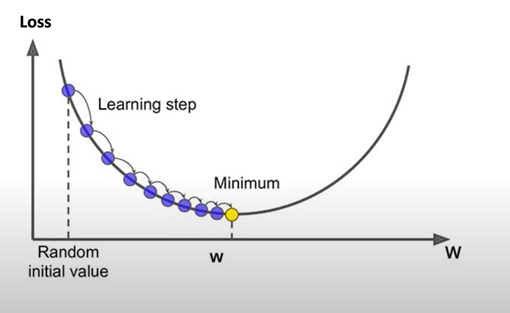
\includegraphics[width=\textwidth]{img/GDham1bien.png}
    \caption{GD cho hàm 1 biến}
    \label{fig:image1}
  \end{minipage}
  \hfill
  \begin{minipage}[b]{0.4\textwidth}
    \centering
    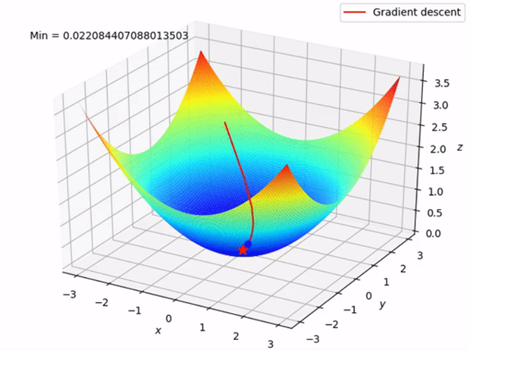
\includegraphics[width=\textwidth]{img/GDhamnhieubien.png}
    \caption{GD cho hàm nhiều biến}
    \label{fig:image2}
  \end{minipage}
  \hfill
\end{figure}
        \item Với learing rate lớn thì ta sẽ tìm được điểm minimum nhanh chóng nhưng với độ chính xác không cao (như hình bên trái chỉ mất 3 epochs)
        \item Với learing rate nhỏ thì ta sẽ tìm được điểm minimum có độ chính xác cao nhưng sẽ mất khá nhiều thời gian.
        \begin{figure}[H]
            \centering
            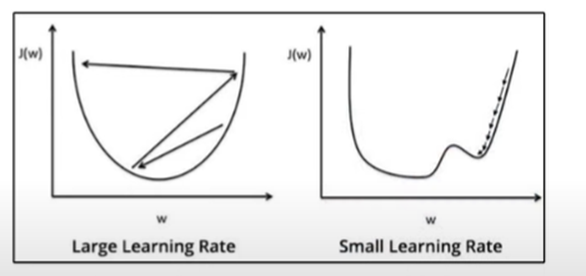
\includegraphics[width=0.75\linewidth]{img/L_S-learning-rate.png}
            \caption{Large và Small Learning Rate}
        \end{figure}
        \item Ưu điểm: thuật toán cơ bản, dễ hiểu, giải quyết được vấn đề tối ưu model bằng cách cập nhật trong số sau mỗi epoch.
        \item Nhược điểm: vì đơn giản và lâu đời nên GD còn nhiều hạn chế như phụ thuộc vào nghiệm khởi tạo ban đầu và learing rate. Ngoài ra tốc độ học quá lớn sẽ khiến cho thuật toán không hội tụ hoặc tốc độ học nhỏ ảnh hưởng đến tốc độ training.   
    \end{itemize}
    
    \item \textbf{Stochastic Gradient Descent (SGD)}
    \begin{itemize}
        \item Stochastic Gradient Descent là một biến thể của Gradient Descent. Thay vì sau mỗi epoch chúng ta sẽ cập nhật trọng số một lần, thì trong mỗi epoch có N điểm dữ liệu, chúng ta sẽ cập nhật trọng số N lần. Nhờ vậy nên SGD sẽ hội tụ rất nhanh chỉ sau vài epoch, ngoài ra SGD có thể phù hợp với online learning.
        \begin{figure}[H]
            \centering
            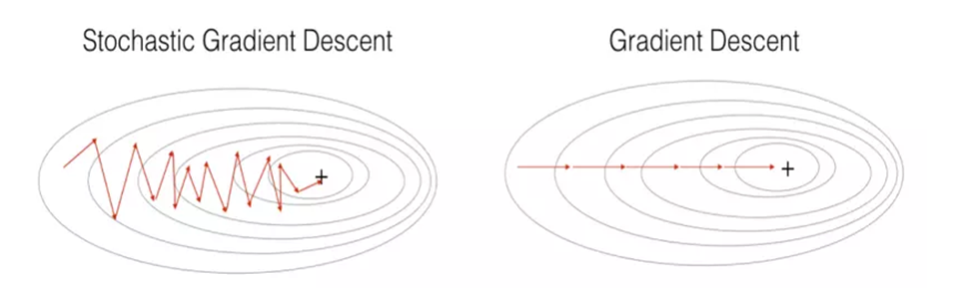
\includegraphics[width=1\linewidth]{img/SGD .png}
            \caption{SGD có đường đi khá zigzag bởi vì 1 điểm dữ liệu không thể đại diện cho toàn bộ dữ liệu}
            
        \end{figure}
        \item Ưu điểm: Thuật toán giải quyết được đối với cơ sở dữ liệu lớn mà GD không làm được.
        \item Nhược điểm: Thuật toán vẫn chưa giải quyết được 2 nhược điểm lớn của GD nên ta phải kết hợp SGD với một số thuật toán khác (Momentum, AdaGrad,...)
    \end{itemize}
    
    \item \textbf{Momentum}
    \begin{itemize}
        \item Để khắc phục thuật toán của GD, người ta sử dụng Momentum.  Để giải thích được Gradient with Momentum thì trước tiên ta nên nhìn dưới góc độ vật lí: Như hình phía dưới, nếu ta thả 2 viên bi tại 2 điểm khác nhau A và B thì viên bị A sẽ trượt xuống điểm C còn viên bi B sẽ trượt xuống điểm D, nhưng ta lại không mong muốn viên bi B sẽ dừng ở điểm D (local minimum) mà sẽ tiếp tục lăn tới điểm C (global minimum). Để thực hiện được điều đó ta phải cấp cho viên bi B 1 vận tốc ban đầu đủ lớn để nó có thể vượt qua điểm E tới điểm C. Dựa vào ý tưởng này người ta xây dựng nên thuật toán Momentum (tức là theo đà tiến tới).
        \begin{figure}[H]
            \centering
            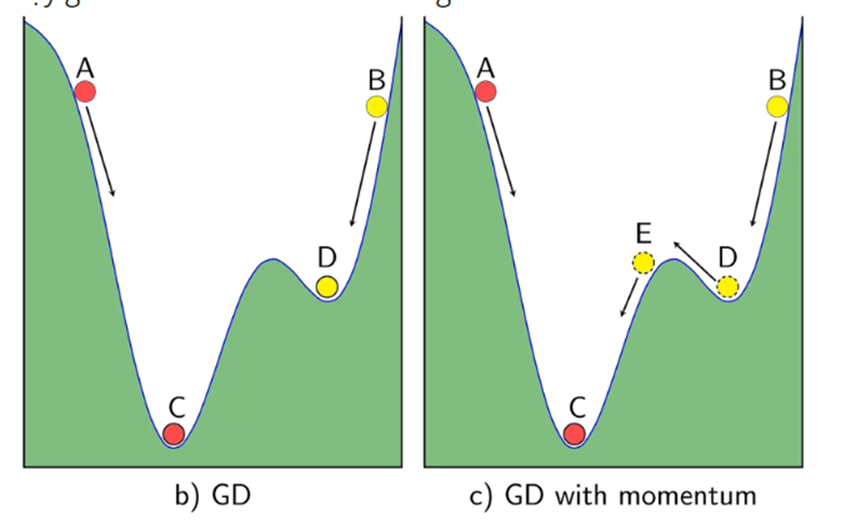
\includegraphics[width=0.75\linewidth]{Momentum.png}
            \caption{Momentum}
            
        \end{figure}
        \begin{center}
                \large $x_{new} = x_{old} -(\gamma \times v + learing\_rate \times gradient)$
            \end{center}
        Trong đó:
        \begin{itemize}
        \item $x_{new}$: tọa độ mới
        \item $x_{old}$: tọa độ cũ
        \item $\gamma$: parameter, thường bằng 0.9
        \item $learning\_rate$: tốc độ học
        \item gradient : đạo hàm của hàm f
        \end{itemize}
        \item Ưu điểm: thuật toán tối ưu giải quyết được vấn đề tiến tới global minimum của GD
        \item Nhược điểm: khi tới gần đích mất khá nhiều thời gian dao động qua lại trước khi dừng hẳn.
    \end{itemize}
    
    \item \textbf{Adagrad}
    \begin{itemize}
        \item Không giống như các thuật toán trước đó với learning rate là hằng số trong quá trình training. Thuật toán Adagrad lại coi learning rate là tham số biến thiên sau mỗi thời điểm t.

        \begin{center}
                \large $\theta_{t + 1} = \theta_{t} - \frac{n}{\sqrt{G_{t}+\epsilon}} \times  g_{t}$
            \end{center}
        Trong đó:
        \begin{itemize}
        \item $n$: hằng số
        \item $g_{t}$: gradient tại thời điểm t
        \item $\epsilon$: hệ số tránh lỗi (chia cho mẫu bằng 0)
        \item $G$: ma trận chéo mà mỗi phần tử trên đường chéo (i,i) là bình phương của đạo hàm vector tham số tại thời điểm t
        \end{itemize}

        
        \item Vấn đề ở đây là giá trị G tăng đơn điệu qua các lần lặp, nên tham số learning rate sẽ giảm đần đến mức không còn cập nhật được nữa.
        \item Ưu điểm: Tránh được việc điều chỉnh learning rate thủ công, chỉ cần để learning rate default là 0.01 thì thuật toán sẽ tự động điều chỉnh.
        \item Nhược điểm: Vì tổng bình biến thiên sẽ lớn dần theo thời gian cho đến khi tốc độ học cực kì nhỏ, làm việc training trở nên đóng băng.
    \end{itemize}
    
    \item \textbf{RMSprop}
    \begin{itemize}
        \item RMSprop là thuật toán giải quyết vấn đề tỷ lệ học giảm dần của Adagard bằng cách chia tỷ lệ học cho trung bình của bình phương gradient
        \begin{center}
                \large $E[g^{2}]_{t} = 0,9E[g^{2}]_{t-1}+0,1g^{2}_{t}$
         \end{center}
         \begin{center}
                \large $\theta_{t + 1} = \theta_{t} - \frac{n}{\sqrt{E[g^{2}]_{t}+\epsilon}} \times  g_{t}$
         \end{center}
        \item Ưu điểm: giải quyến được vấn đề tốc độ học giảm dần của Adagrad
        \item Nhược điểm: có thể cho kết quả nghiệm chỉ là local minimum chứ không đạt được global minimum.
    \end{itemize}
    
    \item \textbf{Adam}
    \begin{itemize}
        \item Adam là thuật toán chủ đạo đang được sử dụng ngày này. Để giải quyết nhược điểm của thuật toán RMSprop, ta có sự kết hợp hoàn hảo với thuật toán Momentum khi có thể đưa kết quả nghiệm đạt được global minimum. Ngược lại, vì thuật toán Momentum có thể đưa ra kết quả nghiệm đạt được global minimum nhưng mất khá nhiều thời gian dao động qua lại trước khi dừng hẳn, ta có thể kết hợp với thuật toán RMSprop để giải quyết được vấn đề tốc độ học giảm dần. Có thể ví Adam như một quả cầu rất nặng và có ma sát, vì có khối lượng nặng nên quả cầu Adam dễ dàng vượt qua local minimum tới global minimum, khi tới global minimum vì có lực ma sát nên nó sẽ dễ dàng dừng lại hơn.  
        \begin{figure}[H]
            \centering
            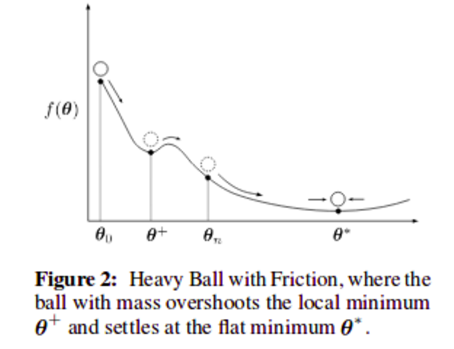
\includegraphics[width=0.5\linewidth]{img/Adam.png}
            \caption{Quả cầu Adam}
            
        \end{figure}
        \item Ưu điểm: tính toán nhanh, tiết kiệm bộ nhớ, rất phù hợp đối với các tập dữ liệu lớn, siêu tham số trực quan và thường yêu cầu ít hoặc không cần điều chỉnh
    \end{itemize}
    
\end{enumerate}




\subsection{Đánh giá mô hình (Test model)}
- Đo lường hiệu suất để đánh giá mô hình là một phần trong quy trình xây dựng máy học. Tất cả các mô hình máy học đều cần \textbf{metric} để đánh giá hiệu suất.
\\- Với \textbf{supervised learning}, có 2 bài toán lớn là \textbf{Regression} và \textbf{Classification}. Sau đây là các \textbf{metric} phổ biến đối với 2 bài toán này: \footnote{Các metric phổ biến dùng trong test model. Cách tính, ý nghĩa từng metric}
\subsubsection{Regression metrics}
Mô hình Regression có đầu ra liên tục (continuous output). Do đó, chúng ta cần một metric dựa trên việc tính toán khoảng cách giữa \textbf{giá trị được dự đoán} (predicted) và \textbf{giá trị thực tế} (ground truth). Các regression metric chủ yếu: \cite{lecture_og}
\begin{itemize}
    \item Mean Absolute Error (MAE)
    \item Mean Squared Error (MSE)
    \item Root Mean Squared Error (RMSE)
\end{itemize}

\begin{enumerate}

\item \textbf{Mean Absolute Error (MAE)} 
\begin{itemize}
\item Giá trị chênh lệch trung bình giữa giá trị thực tế và giá trị được dự đoán bởi mô hình Regression.

\begin{center}
\large $MAE = \frac{1}{N}\sum_{j=1}^{N}\left| y_{i}-\hat{y_{i}} \right|$
\end{center}
Trong đó:
\begin{itemize}
    \item $y_{i}$: giá trị thực tế
    \item $\hat{y_{i}}$: giá trị được dự đoán bởi mô hình Regression
    \item N: số lượng dữ liệu
\end{itemize}
\item Ý nghĩa :
\begin{itemize}
\item MAE có miền giá trị từ $[0,+\infty ]$. 
\item Trên cùng tập dữ liệu, MAE càng nhỏ thì có độ chính xác càng cao.
\item MAE không nhạy cảm với giá trị ngoại lệ (outliers) do việc sử dụng giá trị tuyệt đối.
\item MAE không phản ánh mức độ sai số cụ thể của mô hình. Nó không phân biệt được các lỗi dương và âm, chỉ cho ta biết lỗi trung bình.
\end{itemize}
\end{itemize}
\item\textbf{Mean Squared Error (MSE)}
\begin{itemize}

\item Giá trị trung bình của bình phương độ chênh lệch giữa giá trị mục tiêu và giá trị được dự đoán bởi mô hình Regression.

\begin{center}
\large $MSE = \frac{1}{N}\sum_{j=1}^{N}(y_{i}-\hat{y_{i}})^2$
\end{center}

Trong đó:
\begin{itemize}
    \item $y_{i}$: giá trị thực tế
    \item $\hat{y_{i}}$: giá trị được dự đoán bởi mô hình Regression
    \item N: số lượng dữ liệu
\end{itemize}
\item Ý nghĩa:
\begin{itemize}
\item MSE có miền giá trị từ $[0,+\infty ]$. 
\item Trên cùng tập dữ liệu, MSE càng nhỏ thì có độ chính xác càng cao. 
\item Vì lấy bình phương sai số nên đơn vị của MSE khác với đơn vị của kết quả dự đoán.
\item MSE nhạy cảm với các giá trị ngoại lệ (outliers) do tính bình phương. Các giá trị lớn hơn sẽ có ảnh hưởng lớn hơn đến MSE
\end{itemize}
\end{itemize}

\item \textbf{Root Mean Squared Error (RMSE)}
\begin{itemize}
\item Căn bậc hai giá trị trung bình của bình phương độ chênh lệch giữa giá trị mục tiêu và giá trị được dự đoán bởi mô hình Regression.
\begin{center}
\large $RMSE = \sqrt{\frac{1}{N}\sum_{j=1}^{N}(y_{i}-\hat{y_{i}})^2}$
\end{center}
Trong đó:
\begin{itemize}
    
    \item $y_{i}$: giá trị thực tế
    \item $\hat{y_{i}}$: giá trị được dự đoán bởi mô hình Regression
    \item N: số lượng dữ liệu
\end{itemize}
\item Ý nghĩa:
\begin{itemize}
\item RMSE có miền giá trị từ $[0,+\infty ]$. 
\item Trên cùng tập dữ liệu, RMSE càng nhỏ thì có độ chính xác càng cao. 
\item Việc lấy căn bậc 2 giúp RMSE có cùng đơn vị với kết quả dự đoán, đồng thời làm giá trị RMSE không quá lớn khi số lượng điểm dữ liệu lớn.
\item RMSE cũng như MSE, nhạy cảm với các giá trị ngoại lệ (outliers) do tính bình phương.
\end{itemize}
\end{itemize}

\end{enumerate}

\subsubsection{Classification metrics}
- Các mô hình classification có \textbf{đầu ra rời rạc} (discrete output), vì vậy chúng ta cần metric so sánh các lớp rời rạc dưới một dạng nào đó.\\
- Các classification metric đều đánh giá hiệu suất của mô hình và cho biết mức độ phân loại tốt hay xấu, nhưng mỗi metric lại đánh giá mô hình theo một cách khác nhau.\\
- Các classification metric chủ yếu:
\begin{itemize}
    \item Accuracy
    \item Precision and Recall
    \item F1-score
    \item AU-ROC
\end{itemize}

\textbf{Confusion matrix} \cite{mlwiki} \cite{aiuit} là một kỹ thuật đánh giá hiệu năng của mô hình cho các bài toán phân lớp. Confusion matrix là một ma trận thể hiện số lượng điểm dữ liệu thuộc vào một class và được dự đoán thuộc vào class.\\
\textbf{Confusion matrix} cung cấp thêm thông tin về tỉ lệ phân lớp đúng giữa các lớp, hay giúp phát hiện các lớp có tỉ lệ phân lớp nhầm cao nhờ vào các khái niệm True (False) Positive (Negative)\\

\begin{figure}[H]
    \centering
    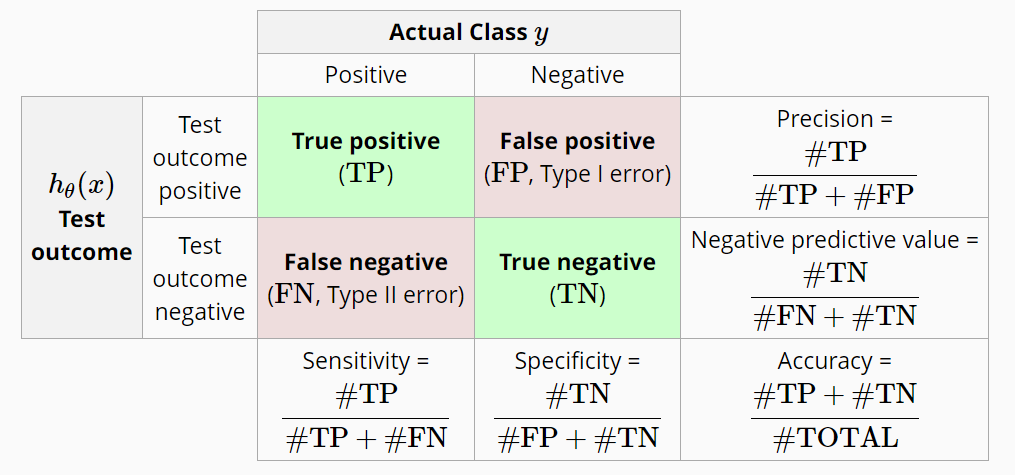
\includegraphics[width=1\linewidth]{img/binary_classifiers.png}
    \caption{Confusion matrix}
\end{figure}

\begin{itemize}
\item \textbf{True positive (TP):} Đối tượng ở lớp Positive, mô hình phân đối tượng vào lớp Positive (dự đoán đúng).
\item \textbf{True negative (TN):} Đối tượng ở lớp Negative, mô hình phân đối tượng vào lớp Negative (dự đoán đúng).
\item \textbf{False positive (FP):} Đối tượng ở lớp Negative, mô hình phân đối tượng vào lớp Positive (dự đoán sai).
\item \textbf{False negative (FN):} Đối tượng ở lớp Positive, mô hình phân đối tượng vào lớp Negative (dự đoán sai).
\end{itemize}
\begin{enumerate}
    \item \textbf{Accuracy} \cite{accuracy} 
    \begin{itemize}
        \item Accuracy (độ chính xác) đánh giá mô hình thường xuyên dự đoán đúng đến mức nào. 
        \item Accuracy là tỉ lệ giữa số điểm dữ liệu được dự đoán đúng và tổng số điểm dữ liệu.
        \item Accuracy lộ rõ hạn chế khi được sử dụng trên bộ dữ liệu không cân bằng (imbalanced dataset). Mô hình có thể đạt accuracy cao khi phân loại dữ liệu vào các lớp đa số.
        \begin{center}
        \large $Accuracy = \frac{Number\ of\ correct\ predictions }{Total\ number\ of\ predictions}$
        \end{center}
        \begin{center}
        \large $Accuracy = \frac{TP + TN}{TP + TN + FP + FN}$
        \end{center}
    \end{itemize}
    
    \item \textbf{Precision} \cite{precision_recall} 
     \begin{itemize}
        \item \textbf{Precision} (Positive Predictive Value): (True Positives) / (All Positive Predictions)
        \begin{center}
        \large $P = Precision = \frac{TP}{TP + FP}$
        \end{center}
        \item Ý nghĩa: "Khi mô hình dự đoán một mẫu là Positive, thì có bao nhiêu tỉ lệ mẫu đó thực sự là Positive?" Nếu Precision cao, tức là tỷ lệ dự đoán Positive đúng của mô hình là cao, và mô hình có khả năng phân loại Positive tốt.
    \end{itemize}

    \item \textbf{Recall} \cite{precision_recall} 
    \begin{itemize}
        \item \textbf{Recall} (True Positive Rate): (True Positives) / (All Actual Positives)
        \begin{center}
        \large $R = Recall = \frac{TP}{TP + FN}$
        \end{center}
        \item Ý nghĩa: "Khi có một mẫu Positive, thì có bao nhiêu tỉ lệ mẫu đó được mô hình dự đoán đúng?" Nếu Recall cao, tức là mô hình có khả năng phát hiện các mẫu Positive tốt.
    \end{itemize}

    \item \textbf{F Measure} \cite{fmeasure}
    \begin{itemize}
        \item \textbf{F-score}: là phép đo đánh giá hiệu suất của mô hình bằng cách kết hợp giữa precision P và recall R
        \begin{center}
        \large $F_\beta = \frac{(\beta^{2} + 1)\times P \times R}{\beta^{2}\times P + R}$
        \end{center}
        \begin{itemize}
            \item Khi $\beta$ tiến đến 0, độ ảnh hưởng của P sẽ càng lớn.
            \item Khi $\beta$ tiến đến $\infty $, độ ảnh hưởng của R sẽ càng lớn.
            \item Ý nghĩa: Sử dụng cả Precision và Recall để đánh giá hiệu suất mô hình.
        \end{itemize}
        \item \textbf{$F_1$-score:} Khi $\beta = 1$, ta được $F_1$-score
        \begin{center}
        \large $F_1 = 2 \frac{P \times R}{P + R}$
        \end{center}
        \begin{itemize}
            \item $F_1$-score: là trung bình điều hòa của precision P và recall R
            \item Ý nghĩa: Precision và Recall có mức độ quan trọng tương đương và cần metric đánh giá hiệu suất tổng thể của mô hình phân loại.
        \end{itemize}
    \end{itemize}

        \item \textbf{ROC Curve, AUC} \cite{roc_auc}
    \begin{itemize}
        \item \textbf{ROC curve:} Đường cong ROC (Receiver Operating Characteristic curve) là biểu đồ hiển thị hiệu suất của mô hình classification ở tất cả các ngưỡng phân loại (classification thresholds). Đường cong này vẽ hai tham số: 
        \begin{enumerate}
            \item True Positive Rate (TPR) - hay còn được gọi là Recall:
            \begin{center}
             \large $TPR = \frac{TP}{TP + FN}$
            \end{center}
            \item False Positive Rate (FPR):
            \begin{center}
             \large $FPR = \frac{FP}{FP + TN}$
            \end{center}
        \end{enumerate}
        Đường cong ROC vẽ đồ thị TPR so với FPR ở các ngưỡng phân loại khác nhau. Việc giảm ngưỡng phân loại sẽ phân loại nhiều mục hơn thành Positive, do đó làm tăng cả kết quả False Positive và kết quả True Positives thực sự. Hình dưới đây cho thấy một đường cong ROC điển hình:
        \begin{figure}[H]
            \centering
            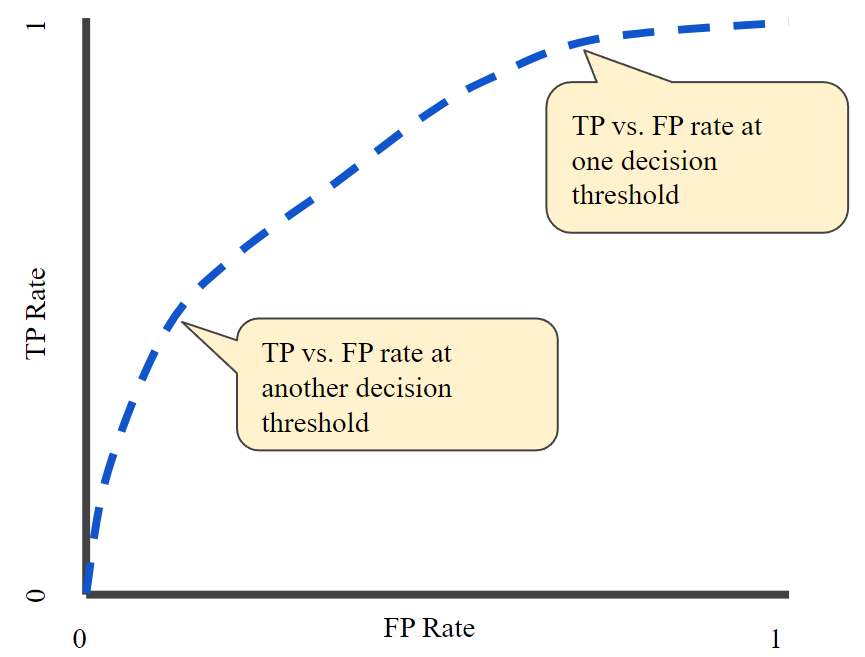
\includegraphics[width=0.5\linewidth]{img/ROC.png}
            \caption{ROC curve}
        \end{figure}
        \item \textbf{AUC:} Diện tích dưới đường cong ROC (Area Under the ROC Curve). AUC đo toàn bộ diện tích hai chiều bên dưới toàn bộ đường cong ROC từ (0,0) đến (1,1) - hay là phép tính tích phân của đường cong ROC từ 0 đến 1.
        \begin{center}
        \large $\int_{0}^{1} ROC(x)dx$
        \end{center}
        \begin{figure}[H]
            \centering
            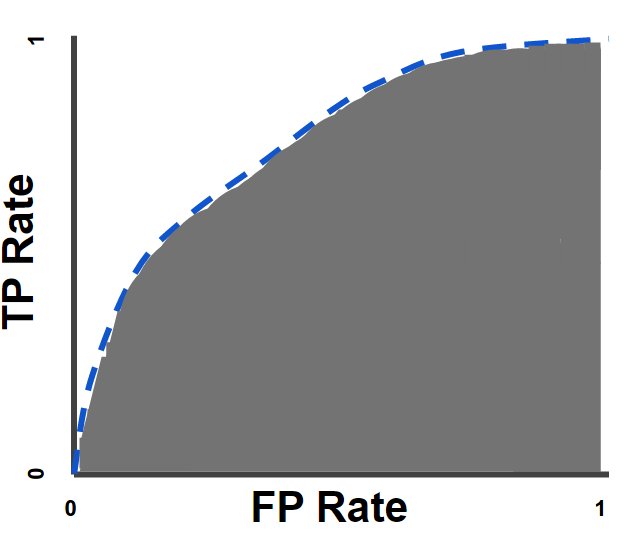
\includegraphics[width=0.5\linewidth]{img/AUC.png}
            \caption{AUC}
        \end{figure}
    \item \textbf{Ý nghĩa:} AUC có giá trị từ 0 đến 1. Với $AUC = 0$, mô hình dự đoán sai 100\%; với $AUC = 1$, mô hình dự đoán đúng 100\%.
    \begin{itemize}
        \item AUC không phụ thuộc vào tỷ lệ \textbf{(scale-invariant)}. AUC đo lường mức độ xếp hạng chính xác của các dự đoán, không phụ thuộc vào giá trị tuyệt đối của chúng.
        \item AUC không phụ thuộc vào ngưỡng phân loại \textbf{(classification-threshold-invariant)}. AUC đo lường chất lượng của các dự đoán mô hình bất kể ngưỡng phân loại được chọn
    \end{itemize}
    \end{itemize}
    
\end{enumerate}
